\documentclass[lettersize,journal]{IEEEtran}
\usepackage{xcolor}
\usepackage{array}
\usepackage{colortbl}
\definecolor{ceblue}{rgb}{.608,.761,.902}
\definecolor{cellblue}{RGB}{102,178,255}
\usepackage{graphicx}
\usepackage{hyperref}
\usepackage{indentfirst}
\usepackage{multirow}
\usepackage{booktabs}
\usepackage{makecell}
\usepackage{url}
\usepackage{cite}
\usepackage{amsmath}
\usepackage{amssymb}
\usepackage{amsfonts}
\usepackage{threeparttable}
\usepackage{tabularx}
\usepackage{longtable}
\usepackage{float}
\usepackage{algorithm}
\usepackage{algorithmicx}
\usepackage{algpseudocode}
\usepackage{subfigure}
\usepackage{subcaption}
\usepackage{tikz,xcolor,hyperref}
\graphicspath{{figures/}}
\hyphenation{op-tical net-works semi-conduc-tor}

\definecolor{lime}{HTML}{A6CE39}
\DeclareRobustCommand{\orcidicon}{%
  
\begin{tikzpicture}
    \draw[lime, fill=lime] (0,0) circle [radius=0.16]
      node[white] {{\fontfamily{qag}\selectfont \tiny ID}};
    \draw[white, fill=white] (-0.0625,0.095) circle [radius=0.007];
  \end{tikzpicture}
  \hspace{-2mm}
}
\foreach \x in {A,...,Z}{%
  \expandafter\xdef\csname orcid\x\endcsname{\noexpand\href{https://orcid.org/\csname orcidauthor\x\endcsname}{\noexpand\orcidicon}}
}

\newcommand{\orcidauthorA}{0000-0002-1986-7144}
\newcommand{\orcidauthorL}{0000-0001-5755-7115}
\newcommand{\orcidauthorN}{0000-0003-2962-192X}
\newcommand{\orcidauthorZ}{0000-0002-6851-0117}
\newcommand{\orcidauthorP}{0000-0002-6747-6367}
\newcommand{\orcidauthorH}{0000-0002-5883-3780}
\newcommand{\orcidauthorB}{0000-0001-8861-5461}
\newcommand{\orcidauthorW}{0000-0002-5074-1363}

\begin{document}
\title{Leakage-Audited Metadata-Only Intrusion Detection for Encrypted MQTT-Based IoT Traffic}

\author{
Dun Li\orcidA{},
Hongzhi Li\orcidH{},
Noel Crespi\orcidN{},
Wei Liang\orcidW{}

\thanks{
Dun Li is with the Department of Industrial Engineering, Tsinghua University, China, and Samovar, Telecom SudParis, Institut Polytechnique de Paris, 91120 Palaiseau, France. E-mail:lidunshmtu@outlook.com
}

\thanks{
Hongzhi Li is with the College of Big Data and Artificial Intelligence, Chizhou University, Chizhou 247100, China. Email: pickpickup@sohu.com
}

\thanks{
Noel Crespi is with Samovar, Telecom SudParis, Institut Polytechnique de Paris, 91120 Palaiseau, France. Email: noel.crespi@mines-telecom.fr
}

\thanks{
Wei Liang is with the School of Computer Science and Engineering, Hunan University of Science and Technology, and Hunan Key Laboratory for Service Computing and Novel Software Technology, China. E-mail: wliang@hnust.edu.cn
}

\thanks{
Corresponding Authors: Noel Crespi, Hongzhi Li}
}

\markboth{IEEE Internet of Things Journal,~Vol.~XX, No.~XX, 2026}%
{Li \MakeLowercase{\textit{et al.}}: Leakage-Audited Metadata-Only MQTT IDS}

\maketitle

\begin{abstract}
MQTT-based Internet of Things (IoT) deployments require intrusion detection mechanisms that remain useful when payload inspection is unavailable. Payload encryption, Transport Layer Security (TLS), and privacy constraints make payload-, topic-, credential-, and client-identifier-based intrusion detection difficult to justify in operational monitoring. This paper presents LAM-MQTT, a leakage-audited metadata-only evaluation framework for encrypted MQTT intrusion detection. The framework separates hard leakage fields from legitimate encrypted-flow metadata and evaluates audited, conservative, and common cross-dataset feature policies on MQTTEEB-D, MQTT-IoT-IDS2020, and IoT-23. The results show that encrypted-flow metadata supports effective within-dataset detection: MQTT-IoT-IDS2020 audited metadata reaches 0.9991 Macro F1, conservative sensitivity reduces this result to 0.9684, and MQTTEEB-D strict 5~s flow-window metadata reaches 0.8925. However, MQTT-to-MQTT transfer is asymmetric and window-dependent, and IoT-23 external robustness remains modest. Metadata-only IDS is therefore useful under cryptographic observability constraints, but it is not a replacement for cryptographic authentication, access control, or protocol hardening.
\end{abstract}

\begin{IEEEkeywords}
Encrypted traffic analysis, intrusion detection, leakage audit, metadata-only monitoring, MQTT, IoT security.
\end{IEEEkeywords}

\section{Introduction}
\label{sec:introduction}
\IEEEPARstart{M}{essage} Queuing Telemetry Transport (MQTT) is a lightweight publish-subscribe protocol widely used in IoT and Industrial Internet of Things (IIoT) environments \cite{mqtt5,sisinni2018industrial}. MQTT clients publish telemetry to a broker, while subscribers receive messages through topic-based routing. This architecture is attractive for resource-constrained devices because it decouples producers and consumers and reduces communication overhead. It also creates an operational security challenge: compromised clients, abnormal publish/subscribe patterns, denial-of-service behavior, brute-force attempts, and malformed protocol interactions can all appear in broker-mediated traffic. These behaviors are often reflected in connection dynamics before they are visible as application-level failures.

In practical deployments, MQTT monitoring is often positioned at the broker, gateway, or network edge rather than inside each constrained device. Such monitors may observe connection behavior and packet dynamics, but they cannot necessarily inspect application semantics. This creates a gap between conventional intrusion detection features, which may assume access to protocol content or endpoint identifiers, and what is actually available in privacy-preserving or encrypted deployments. Similar observability gaps have been studied in encrypted traffic analysis, where protected channels can still expose measurable trace structure \cite{dyer2012peekaboo}.

The monitoring setting is increasingly constrained by encryption and privacy requirements. TLS protects application content in transit \cite{rfc8446}; privacy policies and deployment boundaries may also prevent inspection of raw payloads, raw topic strings, usernames, passwords, client identifiers, and raw IP identities. Intrusion detection systems (IDSs) that rely on such fields can therefore be difficult to deploy, reproduce, or justify. Website fingerprinting and modern encrypted-traffic representation learning further show that packet length, timing, and sequence regularities can remain informative even when content is hidden \cite{hayes2016kfingerprinting,lin2022etbert}. This motivates metadata-only detection: instead of inspecting content, a detector can use flow duration, packet counts, byte statistics, packet-size statistics, inter-arrival-time (IAT) statistics, rates, burstiness, and TCP flag counts, a direction consistent with prior flow and encrypted-traffic analysis \cite{karagiannis2005blinc,drapergil2016vpn}.

Fig.~\ref{fig:motivation} illustrates this encrypted MQTT monitoring setting.
\begin{figure*}[!t]
  \centering
  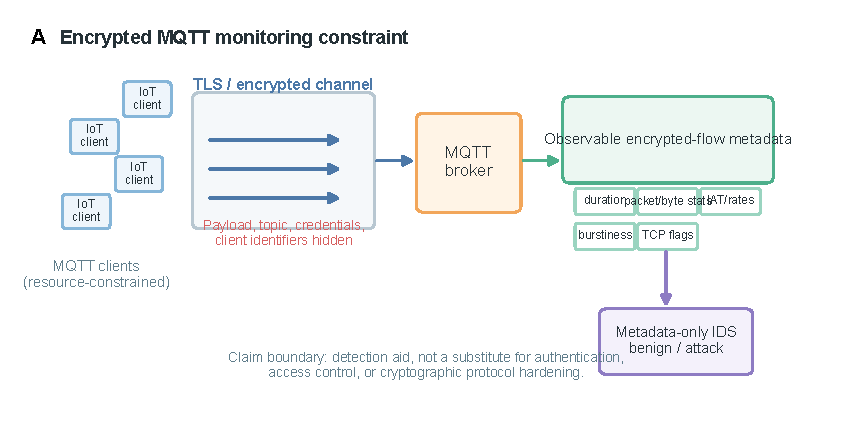
\includegraphics[width=\textwidth]{figures/Fig1_problem_motivation.pdf}
  \caption{Cryptographic observability boundary for metadata-only IDS under encrypted MQTT monitoring. Payloads, topics, credentials, client identities, raw IP identities, and exact timestamps are excluded, while encrypted-flow metadata remains observable.}
  \label{fig:motivation}
\end{figure*}

The central question is therefore not whether metadata can replace protocol security, but whether a carefully bounded metadata signal can provide an additional detection layer. Such a layer is complementary to access-control and data-governance mechanisms for IIoT, including smart-contract and proof-inspired access-control schemes \cite{li2025hyperiiot,li2025dpsiiot}. Answering this question requires an explicit observability model: features should be admitted only when they would plausibly remain available without decrypting traffic or collecting sensitive raw fields.

Metadata-only detection is useful but risky. It is useful because many attacks alter observable communication dynamics even when payloads are encrypted. It is risky because public security datasets can contain artifacts that inflate within-dataset scores, including labels, attack-category fields, scenario names, source-file indicators, exact timestamps, and raw identity fields. Security-ML evaluation critiques have repeatedly warned that hidden bias and unrealistic experimental design can lead to overconfident claims \cite{arp2022dosdonts,pendlebury2019tesseract}. Random within-dataset splits can further overestimate deployment performance when dataset-specific patterns are shared between training and test partitions. A credible evaluation must therefore distinguish legitimate encrypted-flow metadata from hard leakage, and it must evaluate robustness beyond a single random split.

This paper makes four contributions.
\begin{itemize}
  \item We formulate encrypted MQTT intrusion detection under cryptographic observability constraints.
  \item We develop a leakage-audited metadata construction procedure that separates hard leakage from legitimate encrypted-flow metadata.
  \item We evaluate audited, conservative, and common cross-dataset feature policies on MQTTEEB-D, MQTT-IoT-IDS2020, and IoT-23.
  \item We show that metadata-only detection is effective within dataset, but cross-dataset transfer is asymmetric and external IoT robustness remains limited.
\end{itemize}

The remainder of this paper is organized as follows. Section~\ref{sec:related} reviews related work, Section~\ref{sec:methodology} presents LAM-MQTT, Section~\ref{sec:results} reports the experiments and findings, and Section~\ref{sec:conclusion} concludes the paper.

\section{Related Work}
\label{sec:related}
\subsection{MQTT and IoT Intrusion Detection}
Machine-learning-based IoT intrusion detection has been studied extensively because IoT deployments combine constrained devices, heterogeneous protocols, and exposed network services \cite{algaradi2020survey,hussain2020machine,hodo2017taxonomy}. Broader IIoT security work has also emphasized trustworthy data exchange, blockchain-supported governance, and digital-twin security as complementary protection layers \cite{li2025blockchaindt}. MQTT is a particularly important protocol in this context. Its broker-mediated publish-subscribe model is efficient, but weak authentication, insecure deployment choices, broker exposure, and abnormal publish/subscribe behavior can produce detectable network-level symptoms. MQTT-focused benchmarks, including MQTTset, have made attack detection experimentally tractable, but their use still requires careful feature auditing \cite{vaccari2020mqttset}.

Several broader IoT and IIoT corpora provide additional context. CICIoT2023, ToN-IoT, Bot-IoT, N-BaIoT, and Edge-IIoTset cover different attack surfaces, device types, and collection environments \cite{ciciot2023,alsaedi2020toniot,koroniotis2019botiot,meidan2018nbaiot,ferrag2022edgeiiotset}. IoT botnet studies, including Mirai analyses, further show that compromised devices can generate large-scale network effects that are visible in timing, volume, and connection behavior \cite{antonakakis2017mirai,kolias2017mirai}. These corpora support benchmarking, but they also differ substantially in capture setup, labels, feature definitions, and attack distributions.

\subsection{Encrypted Traffic Analysis and Metadata-Only Monitoring}
Encrypted traffic analysis has long used timing, direction, and size metadata when payload inspection is unavailable. Classical traffic-classification work used Bayesian models and flow statistics to infer application classes without relying only on port numbers \cite{moore2005bayesian}. Mobile and encrypted-application fingerprinting work further demonstrated that packet sizes and timing can reveal behavioral structure even when content is protected \cite{conti2016android,taylor2016appscanner}. Deep learning studies later explored packet-sequence and representation-learning approaches for encrypted traffic classification \cite{lotfollahi2020deeppacket,rezaei2019overview,aceto2019mimetic,wang2017encryptedcnn}. IoT traffic classifiers also use convolutional and recurrent models over flow or packet representations \cite{lopezmartin2017traffic,sivanathan2019iotdevices}.

This paper differs from payload-oriented and packet-content approaches by enforcing a metadata-only boundary. The goal is not to decrypt TLS, bypass cryptographic protection, or replace authentication and access control. Instead, the objective is to test how far legitimate encrypted-flow metadata can support IDS decisions when content and raw identities are not used.

\subsection{Dataset Leakage, Dataset Bias, and Cross-Dataset IDS Evaluation}
Network IDS evaluation is vulnerable to closed-world assumptions. Sommer and Paxson emphasized the gap between machine-learning success in controlled settings and operational network intrusion detection \cite{sommer2010outside}. Dataset surveys similarly show that benchmark suitability depends on capture environment, labeling, feature construction, attack diversity, and temporal realism \cite{ring2019survey}. More generally, dataset shift and transfer-learning studies show that training and test distributions often differ in real deployments \cite{quionero2009datasetshift,pan2010transfer}.

For metadata-only MQTT IDS, this means that a high random-split score is not sufficient. Features must be checked for leakage, and models should be evaluated under conservative sensitivity, cross-dataset transfer, and external robustness settings. Hard leakage and dataset-specific artifacts must be separated from legitimate metadata that is predictive because attack behavior changes flow dynamics.

\subsection{Public IoT Security Datasets and MQTT Benchmarks}
Public security datasets have shaped IDS evaluation, including CICIDS2017 and UNSW-NB15 for general network intrusion detection \cite{sharafaldin2018cicids,moustafa2015unsw}. Flow-based IDS surveys and online anomaly detectors such as Kitsune reinforce the practical value of compact network metadata for high-speed or resource-constrained monitoring \cite{sperotto2010flow,umer2017flow,garcia2009anomaly,ahmed2016survey,mirsky2018kitsune}. These datasets and methods are complementary rather than interchangeable. In particular, external IoT datasets should not be treated as MQTT benchmarks unless their capture protocol and feature space support that interpretation.

\section{Methodology}
\label{sec:methodology}
\subsection{LAM-MQTT Overview}
We define LAM-MQTT, a Leakage-Audited Metadata Framework for Encrypted MQTT Intrusion Detection. The framework is designed to evaluate what can be learned from metadata that remains observable under encryption or privacy-constrained monitoring. Fig.~\ref{fig:framework} summarizes the pipeline.

\begin{figure*}[!t]
  \centering
  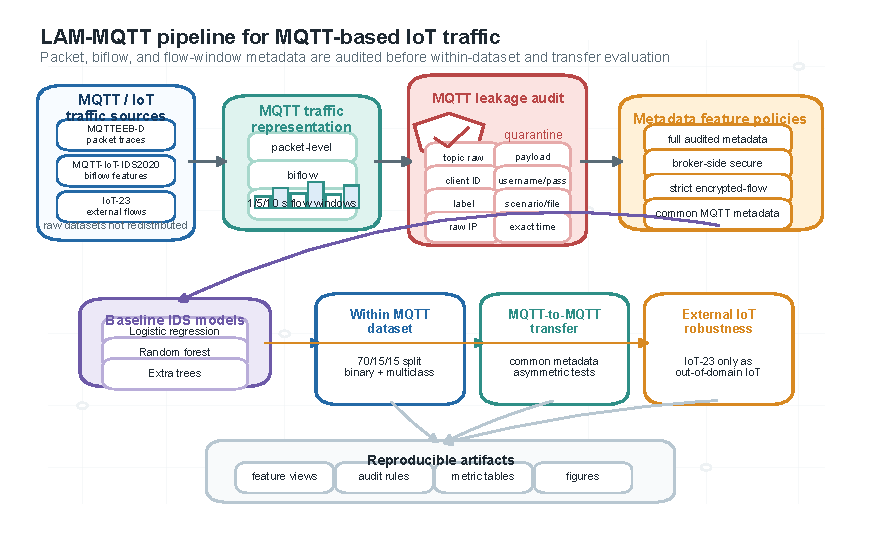
\includegraphics[width=\textwidth]{figures/Fig2_framework.pdf}
  \caption{LAM-MQTT leakage-audited experimental framework. The pipeline ingests public datasets, normalizes labels, quarantines hard leakage fields, constructs observability-aware feature policies, trains baseline learners, and evaluates within-dataset, MQTT-to-MQTT, and external IoT robustness settings.}
  \label{fig:framework}
\end{figure*}

The pipeline contains six steps. First, datasets are ingested and labels are normalized for binary and multiclass tasks. Second, hard leakage fields are excluded. Third, cryptographic observability views are constructed. Fourth, a conservative sensitivity policy removes additional highly discriminative metadata. Fifth, a common cross-dataset metadata space aligns MQTT datasets for transfer evaluation. Sixth, within-dataset, cross-dataset, external robustness, feature-family, and multi-seed protocols are evaluated.

\subsection{Dataset Ingestion and Label Normalization}
The evaluation uses MQTTEEB-D \cite{mqtteebd2025}, MQTT-IoT-IDS2020 \cite{hindy2020mqttiot}, and IoT-23 \cite{iot23}. MQTTEEB-D is evaluated in two granularities. The packet-level strict view is retained as a weak baseline because it contains only a very small strict metadata set. The flow-window strict view is the main encrypted-flow representation for MQTTEEB-D and is evaluated at 1~s, 5~s, and 10~s windows. MQTT-IoT-IDS2020 is evaluated using biflow features. IoT-23 is used only for external IoT robustness validation. Labels are normalized into binary and multiclass targets where appropriate; no label or attack-name field is retained as a model input.

\subsection{Hard Leakage Exclusion}
LAM-MQTT removes hard leakage before model training. The removed categories include labels, attack categories, scenario names, source-file indicators, raw IP identities, exact timestamps, client identifiers, usernames, passwords, payload content, and raw topic strings. These fields either encode the target directly, identify the capture or scenario, or violate encrypted/privacy-constrained deployment assumptions.

The framework retains legitimate metadata: duration, packet counts, byte statistics, packet-size statistics, IAT statistics, rates, burstiness, and TCP flag counts. High single-feature discriminative ability does not automatically imply leakage. A flow statistic can be highly predictive because an attack changes communication timing or volume; such a feature is treated as legitimate metadata unless it encodes labels, identities, scenarios, or unavailable content.

\subsection{Feature Policy Definitions}
Let $\mathcal{X}$ denote the set of candidate fields after dataset parsing. LAM-MQTT defines a hard leakage set $\mathcal{H}$ containing labels, attack categories, scenario names, source files, raw IP identities, exact timestamps, client identifiers, usernames, passwords, payload content, and raw topic strings. It also defines a legitimate metadata set $\mathcal{M}$ containing duration, packet and byte statistics, packet-size statistics, IAT statistics, rates, burstiness, and TCP flags. The three feature policies are
\begin{align}
\mathcal{F}_{\mathrm{main}} &= \mathcal{X} \setminus \mathcal{H},\\
\mathcal{F}_{\mathrm{cons}} &= \mathcal{F}_{\mathrm{main}} \setminus \mathcal{S},\\
\mathcal{F}_{\mathrm{common}}^{a,b} &= \mathcal{F}_{\mathrm{main}}^{a} \cap \mathcal{F}_{\mathrm{main}}^{b} \cap \mathcal{M}.
\end{align}
Here, $\mathcal{S}$ is the set of additional highly discriminative metadata removed only for conservative sensitivity analysis. The common policy $\mathcal{F}_{\mathrm{common}}^{a,b}$ is applied after semantic alignment of feature names across source dataset $a$ and target dataset $b$. High single-feature predictiveness alone does not move a feature from $\mathcal{M}$ to $\mathcal{H}$; a metadata feature is excluded as hard leakage only when it directly encodes the target, a capture artifact, raw identity, exact time, or content unavailable under the encrypted monitoring model.

\begin{algorithm}[!t]
\caption{LAM-MQTT feature policy construction}
\label{alg:lammqtt}
\begin{algorithmic}[1]
\Require Candidate fields $\mathcal{X}$, leakage rules $\mathcal{H}$, metadata vocabulary $\mathcal{M}$
\Ensure $\mathcal{F}_{\mathrm{main}}$, $\mathcal{F}_{\mathrm{cons}}$, $\mathcal{F}_{\mathrm{common}}$
\State Remove all hard leakage fields in $\mathcal{H}$ from $\mathcal{X}$
\State Set $\mathcal{F}_{\mathrm{main}} \gets \mathcal{X} \setminus \mathcal{H}$
\State Build observability views from fields consistent with $\mathcal{M}$
\State Identify $\mathcal{S}$ for conservative sensitivity without relabeling $\mathcal{S}$ as leakage
\State Set $\mathcal{F}_{\mathrm{cons}} \gets \mathcal{F}_{\mathrm{main}} \setminus \mathcal{S}$
\State Align semantically equivalent metadata names across datasets
\State Set $\mathcal{F}_{\mathrm{common}}^{a,b} \gets \mathcal{F}_{\mathrm{main}}^{a} \cap \mathcal{F}_{\mathrm{main}}^{b} \cap \mathcal{M}$
\end{algorithmic}
\end{algorithm}

\subsection{Cryptographic Observability Views}
LAM-MQTT constructs three observability views (Fig.~\ref{fig:views}). The full audited view is an upper-bound metadata setting after hard leakage removal. The broker-side secure metadata view represents features plausibly available near the MQTT broker without raw sensitive content. The strict encrypted-flow view contains features expected to remain observable even when payloads and topics are encrypted.

\begin{figure*}[!t]
  \centering
  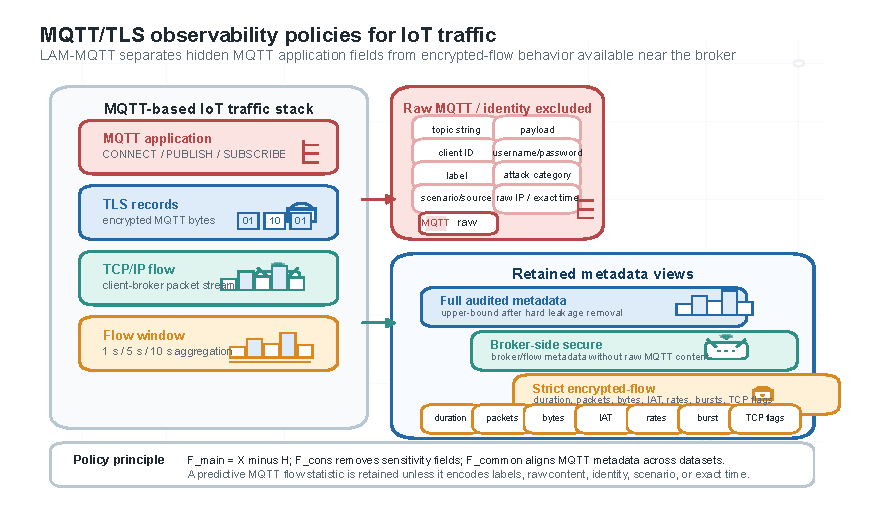
\includegraphics[width=\textwidth]{figures/Fig3_crypto_observability_views.pdf}
  \caption{Cryptographic observability feature policies. Hard leakage and sensitive raw fields are removed before model training, while full audited, broker-side secure, and strict encrypted-flow metadata views retain progressively constrained legitimate metadata.}
  \label{fig:views}
\end{figure*}

\begin{table}[!t]
\centering
\caption{Audited metadata feature counts by dataset and observability view.}
\label{tab:featureviews}
\begin{threeparttable}
\begin{tabular}{lccc}
\toprule
Dataset & Full & Broker & Strict \\
\midrule
MQTTEEB-D & 9 & 9 & 2 \\
MQTT-IoT & 42 & 42 & 42 \\
IoT-23 & 31 & -- & 31 \\
MQTTEEB-D flow 1 s & 15 & 15 & 14 \\
MQTTEEB-D flow 5 s & 15 & 15 & 14 \\
MQTTEEB-D flow 10 s & 15 & 15 & 14 \\
\bottomrule
\end{tabular}
\begin{tablenotes}[flushleft]
\footnotesize
\item Dataset sources: MQTTEEB-D~\cite{mqtteebd2025}; MQTT-IoT-IDS2020~\cite{hindy2020mqttiot}; IoT-23~\cite{iot23}.
\end{tablenotes}
\end{threeparttable}
\end{table}

Table~\ref{tab:featureviews} reports the audited feature counts. For MQTT-to-MQTT transfer, the framework aligns 14 common metadata features: packet count, byte summary statistics, duration, IAT summary statistics, byte and packet rates, and burstiness.

\subsection{Flow-Window Aggregation}
For MQTTEEB-D, packet-level records are additionally aggregated into fixed time windows $\Delta \in \{1,5,10\}$ seconds. Within each window, LAM-MQTT computes duration, packet count, byte summary statistics, IAT summary statistics, byte and packet rates, and burstiness. These flow-window features provide the primary strict encrypted-flow representation for MQTTEEB-D, whereas the packet-level strict view is treated as a weak baseline.

The raw timestamp is used only to assign packet records to windows and to derive duration and IAT statistics. It is not retained as a model input. For binary labels, a window is labeled as attack when any record in the window is labeled as attack. For multiclass labels, the window label follows the majority class within the window, and mixed-label information is used only for aggregation diagnostics.

\subsection{Evaluation Protocol}
The conservative sensitivity policy removes additional highly discriminative metadata to test whether performance depends on a small set of strong flow signals. This policy is a stress test, not the main deployment claim. The evaluated tasks include binary classification and multiclass classification when supported by the dataset labels. The model families include linear and tree-based baselines, with Macro F1 used as the primary metric. Accuracy is reported in the underlying metric tables but is not emphasized because IDS benchmarks are often class-imbalanced \cite{buczak2016survey,khraisat2019survey}.

The primary within-dataset protocol uses a 70/15/15 random stratified split with seed 42. Time-block splits are treated as formal performance only when the resulting test block contains at least two classes; invalid time-block rows are excluded from official performance interpretation. Cross-dataset experiments train on one MQTT dataset view and test on another using common metadata. IoT-23 experiments are treated as external IoT robustness validation rather than MQTT-to-MQTT transfer. The implementation records all processed feature views and metric tables for reproducibility.

\section{Experiments and Results}
\label{sec:results}
\subsection{Finding 1: Audited encrypted-flow metadata supports strong within-dataset detection}
Table~\ref{tab:within} summarizes the main within-dataset results, and Fig.~\ref{fig:within} visualizes Macro F1 for the packet-level MQTTEEB-D and biflow MQTT-IoT audited views. The MQTTEEB-D packet-level and flow-window results are different feature granularities. At packet level, metadata is informative but challenging: the best binary random-stratified result is 0.6549 Macro F1 with full or broker-side metadata, and the strict packet-level weak baseline reaches 0.6450. After flow-window aggregation, the MQTTEEB-D 5~s strict encrypted-flow representation reaches 0.8925 Macro F1. This comparison shows that the 0.6450 and 0.8925 values should not be interpreted as the same setting.

MQTT-IoT-IDS2020 shows much stronger within-dataset separability after hard leakage removal. Audited metadata reaches 0.9991 Macro F1 for binary classification and 0.9992 for multiclass classification across full, broker-side, and strict views. These results demonstrate strong in-distribution separability under the evaluated splits, but they do not imply unconditional deployment generalization.

\begin{table}[!t]
\centering
\caption{Within-dataset Macro F1 under audited metadata. Packet-level and flow-window rows are separate feature granularities.}
\label{tab:within}
\begin{threeparttable}
\begin{tabular}{llll}
\toprule
Dataset/granularity & Task & View & Macro F1 \\
\midrule
MQTTEEB-D packet & binary & full/broker & 0.6549 \\
MQTTEEB-D packet & binary & strict & 0.6450 \\
MQTTEEB-D flow 5 s & binary & strict & 0.8925 \\
MQTTEEB-D packet & multiclass & full/broker & 0.5595 \\
MQTTEEB-D packet & multiclass & strict & 0.5327 \\
MQTT-IoT biflow & binary & all views & 0.9991 \\
MQTT-IoT biflow & multiclass & all views & 0.9992 \\
\bottomrule
\end{tabular}
\begin{tablenotes}[flushleft]
\footnotesize
\item Dataset sources: MQTTEEB-D~\cite{mqtteebd2025}; MQTT-IoT-IDS2020~\cite{hindy2020mqttiot}.
\end{tablenotes}
\end{threeparttable}
\end{table}

\begin{figure}[!t]
  \centering
  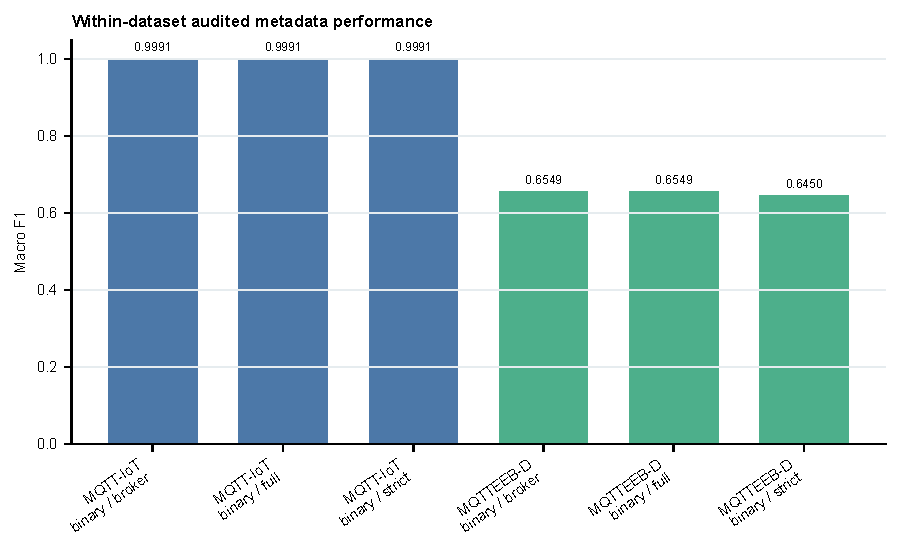
\includegraphics[width=\linewidth]{figures/Fig4_within_dataset_main_macro_f1.pdf}
  \caption{Within-dataset Macro F1 for packet-level MQTTEEB-D and MQTT-IoT biflow audited views. MQTTEEB-D flow-window results are reported separately.}
  \label{fig:within}
\end{figure}

\subsection{Finding 2: Conservative sensitivity reduces MQTT-IoT performance}
The conservative policy reduces MQTT-IoT strict features from 42 to 14. Binary Macro F1 decreases from 0.9991 under the audited main policy to 0.9684, and multiclass Macro F1 decreases from 0.9992 to 0.9489. This indicates that the most discriminative metadata features drive much of the detection ability. The decrease should be interpreted as sensitivity to removing legitimate flow metadata, not as proof that those metadata fields are label leakage.

\subsection{Finding 3: Crypto-observability ablation favors the MQTTEEB-D 5 s strict flow window}
Table~\ref{tab:crypto} and Fig.~\ref{fig:crypto} report the crypto-observability ablation. For MQTTEEB-D, strict flow-window metadata substantially improves over packet-level strict metadata. The 1~s strict flow view reaches 0.8693 Macro F1, the 5~s strict view reaches 0.8925, and the 10~s strict view reaches 0.8709. Among the tested MQTTEEB-D windows, the 5~s strict view performs best. For MQTT-IoT, audited full, broker-side, and strict encrypted-flow views all reach 0.9991 Macro F1, while the conservative strict view reaches 0.9684.

\begin{table}[!t]
\centering
\caption{Crypto-observability and conservative sensitivity results. Packet-level strict and flow-window strict results are separate feature granularities.}
\label{tab:crypto}
\begin{threeparttable}
\begin{tabular}{llr}
\toprule
Dataset/view & Policy & Macro F1 \\
\midrule
MQTTEEB-D packet & strict & 0.6450 \\
MQTTEEB-D flow 1 s & strict & 0.8693 \\
MQTTEEB-D flow 5 s & strict & 0.8925 \\
MQTTEEB-D flow 10 s & strict & 0.8709 \\
MQTT-IoT biflow & strict audited & 0.9991 \\
MQTT-IoT biflow & conservative & 0.9684 \\
\bottomrule
\end{tabular}
\begin{tablenotes}[flushleft]
\footnotesize
\item Dataset sources: MQTTEEB-D~\cite{mqtteebd2025}; MQTT-IoT-IDS2020~\cite{hindy2020mqttiot}.
\end{tablenotes}
\end{threeparttable}
\end{table}

\begin{figure}[!t]
  \centering
  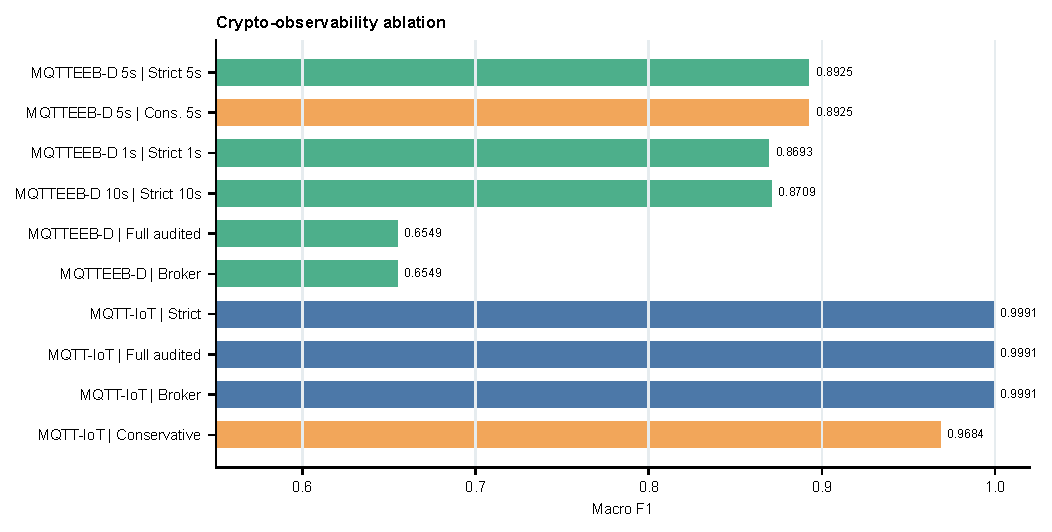
\includegraphics[width=\linewidth]{figures/Fig5_crypto_observability_ablation_revised.pdf}
  \caption{Crypto-observability ablation under audited and conservative feature policies.}
  \label{fig:crypto}
\end{figure}

\subsection{Finding 4: MQTT-to-MQTT transfer is asymmetric and window-dependent}
Table~\ref{tab:cross} and Fig.~\ref{fig:cross} report MQTT-to-MQTT transfer with the 14 common metadata features. Training on MQTT-IoT and testing on MQTTEEB-D flow windows gives 0.6417 Macro F1 for the 1~s window, 0.7312 for the 5~s window, and 0.8172 for the 10~s window. The reverse direction is uneven: MQTTEEB-D 1~s to MQTT-IoT reaches 0.9140, but MQTTEEB-D 5~s and 10~s to MQTT-IoT reach only 0.2735 and 0.2149, respectively. These results support a bounded conclusion: common encrypted-flow metadata can transfer in selected settings, but MQTT-to-MQTT generalization is not uniformly strong.

\begin{table}[!t]
\centering
\caption{MQTT-to-MQTT cross-dataset Macro F1 with 14 common metadata features. MQTTEEB-D rows denote flow-window settings.}
\label{tab:cross}
\begin{threeparttable}
\begin{tabular}{llr}
\toprule
Train & Test & Macro F1 \\
\midrule
MQTT-IoT & MQTTEEB-D 1 s & 0.6417 \\
MQTT-IoT & MQTTEEB-D 5 s & 0.7312 \\
MQTT-IoT & MQTTEEB-D 10 s & 0.8172 \\
MQTTEEB-D 1 s & MQTT-IoT & 0.9140 \\
MQTTEEB-D 5 s & MQTT-IoT & 0.2735 \\
MQTTEEB-D 10 s & MQTT-IoT & 0.2149 \\
\bottomrule
\end{tabular}
\begin{tablenotes}[flushleft]
\footnotesize
\item Dataset sources: MQTTEEB-D~\cite{mqtteebd2025}; MQTT-IoT-IDS2020~\cite{hindy2020mqttiot}.
\end{tablenotes}
\end{threeparttable}
\end{table}

\begin{figure}[!t]
  \centering
  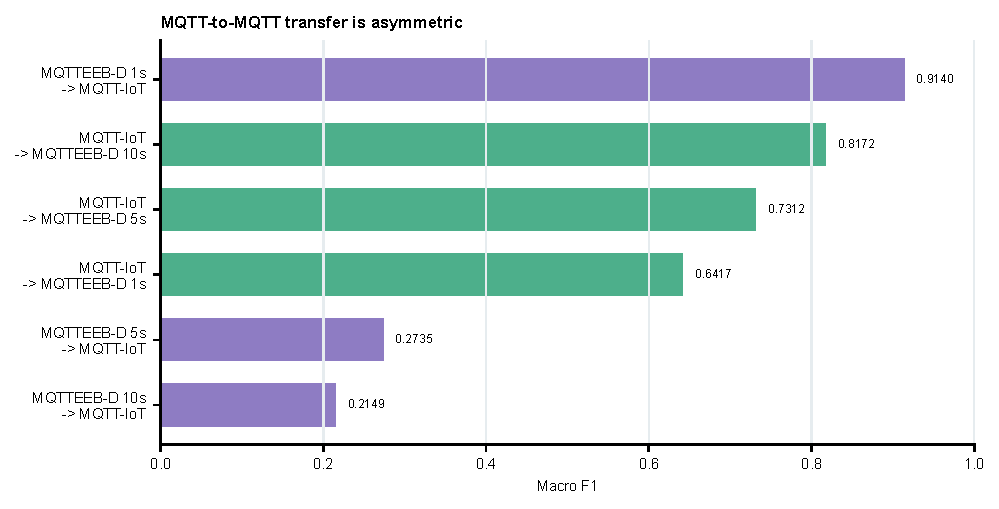
\includegraphics[width=\linewidth]{figures/Fig6_mqtt_to_mqtt_cross_dataset_main.pdf}
  \caption{Bidirectional MQTT-to-MQTT cross-dataset Macro F1 under common encrypted-flow metadata.}
  \label{fig:cross}
\end{figure}

\subsection{Finding 5: IoT-23 external robustness remains modest}
IoT-23 is used only as external IoT robustness validation. MQTTEEB-D 5~s strict metadata transferred to IoT-23 with 0.4720 Macro F1, while MQTT-IoT strict metadata transferred to IoT-23 with 0.5076. These values are modest compared with within-dataset MQTT results and indicate out-of-domain IoT shift.

Feature-family ablation further clarifies the metadata signal. Fig.~\ref{fig:family} shows that byte, IAT, packet-count, rate, burstiness, and TCP-related families carry meaningful information. For MQTT-IoT, all metadata reaches 0.9991, byte statistics alone reach 0.9977, IAT-only reaches 0.9500, packet-count-only reaches 0.9493, rate-only reaches 0.9501, and TCP-flags-only reaches 0.9269. For MQTTEEB-D 5~s strict metadata, all metadata reaches 0.8925, byte statistics alone reach 0.8945, rate features reach 0.8915, IAT-only reaches 0.8755, and packet-count-only reaches 0.8755.

\begin{figure}[!t]
  \centering
  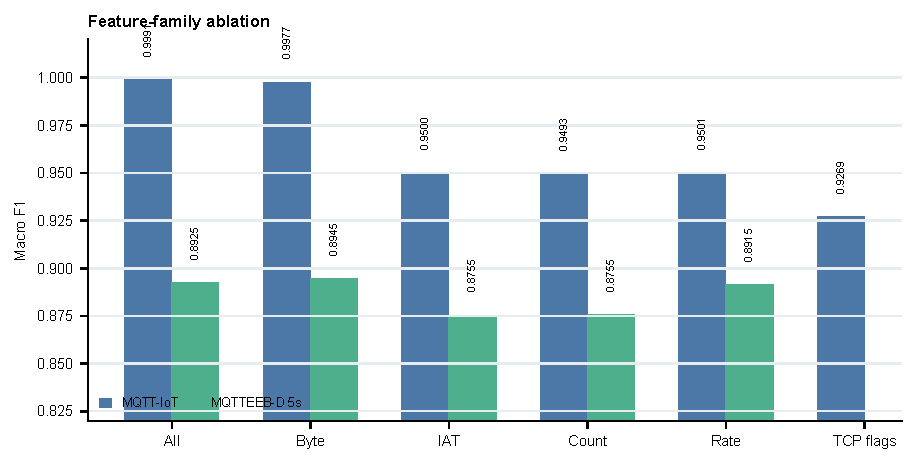
\includegraphics[width=\linewidth]{figures/Fig7_feature_family_ablation.pdf}
  \caption{Feature-family ablation for MQTT-IoT and MQTTEEB-D strict 5~s metadata.}
  \label{fig:family}
\end{figure}

Feature importance should be interpreted with the ablation rather than as causal proof. Fig.~\ref{fig:importance} shows model-level importance for top metadata features. Multi-seed stability is consistent with the main findings: MQTTEEB-D strict 5~s binary reports 0.8862 $\pm$ 0.0051 Macro F1, MQTT-IoT strict binary reports 0.9993 $\pm$ 0.0001, MQTT-IoT to MQTTEEB-D strict 5~s reports 0.7464 $\pm$ 0.0310, and MQTTEEB-D strict 5~s to MQTT-IoT reports 0.1994 $\pm$ 0.0536.

\begin{figure}[!t]
  \centering
  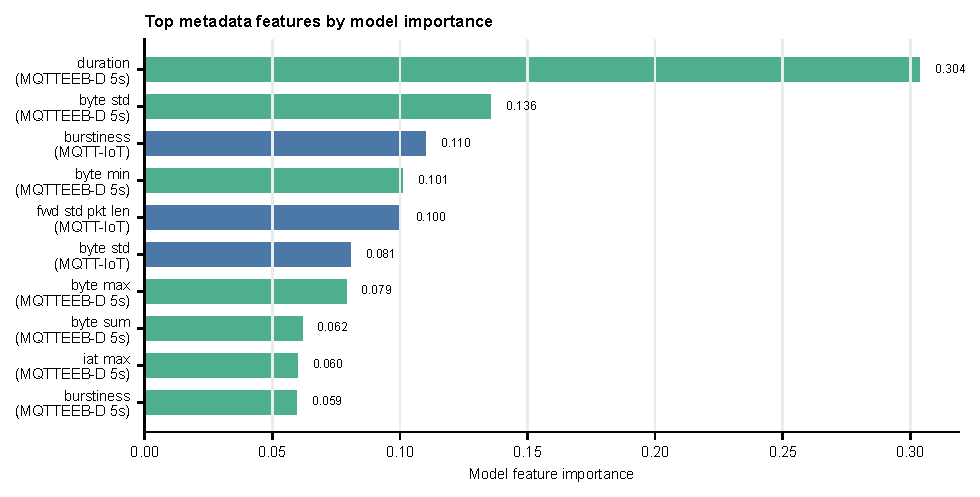
\includegraphics[width=\linewidth]{figures/Fig8_feature_importance.pdf}
  \caption{Model-level feature importance for metadata-based IDS. Importance is model-level evidence and should not be interpreted as causal attribution.}
  \label{fig:importance}
\end{figure}

\section{Conclusion}
\label{sec:conclusion}
This paper presented LAM-MQTT, a leakage-audited metadata-only evaluation framework for encrypted MQTT traffic. The framework removes hard leakage and sensitive raw fields while retaining legitimate encrypted-flow metadata. Within-dataset results show that such metadata can support effective MQTT-IoT attack detection, particularly on MQTT-IoT-IDS2020, while MQTTEEB-D benefits from flow-window construction.

The conservative sensitivity and feature-family ablation indicate that byte statistics, IAT statistics, rates, burstiness, and related flow behavior are core signals under the evaluated settings. These features should not be confused with label leakage solely because they are predictive. At the same time, MQTT-to-MQTT transfer asymmetry and modest IoT-23 robustness indicate operational shift across datasets and deployment contexts.

Future work should evaluate additional MQTT captures, real broker deployments, valid group or time-separated splits, and online edge deployment. Metadata-only IDS should be viewed as a deployment-compatible detection layer under cryptographic observability constraints, not as a replacement for cryptographic authentication, access control, or protocol hardening.

\section*{Data and Code Availability}
The study uses public datasets: MQTTEEB-D, MQTT-IoT-IDS2020, and IoT-23. The source code, configuration files, leakage-audit rules, feature-view construction scripts, processed metric tables, and figure-generation scripts are available at: \url{https://github.com/DunLi-Tsinghua/LAM-MQTT}. The original raw datasets are not redistributed in the repository and should be obtained from their official sources, subject to their respective access and redistribution terms. The implementation records feature views, leakage audit decisions, processed metrics, and figures for reproducibility. The method does not decrypt TLS traffic and does not replace authentication, access control, or protocol hardening. Sensitive raw fields such as payloads, topics, credentials, client identifiers, raw IP identities, and exact timestamps are excluded from model inputs.

\bibliographystyle{IEEEtran}
\bibliography{references}
\end{document}
